\section{Experimentaci\'on}

Como fue previamente mencionado, la idea ser\'a estudiar qu\'e par\'ametros optimizan el c\'alculo de RTO. Para realizar esto, dividiremos la experimentaci\'on en dos etapas.

Durante la primera etapa, analizaremos c\'omo evoluciona la estimaci\'on de RTO en el cliente con distintas combinaciones de $\alpha$ y $\mathcal{B}$ para un delay fijo y probabilidad de p\'erdida de paquetes nula. A partir de esta experimentaci\'on nos quedaremos con 4 combinaciones de $\alpha$ y $\mathcal{B}$ que a nuestro crtierio son los mejores para estimar el RTO.

Durante la segunda etapa, observaremos c\'omo se comportan las combinaciones anteriores. Para ello volveremos a analizar como evoluciona la estimaci\'on de RTO en el cliente pero, esta vez, iremos variando el delay y la probabilidad de p\'erdida de paquetes. 

\subsection{Etapa Inicial: Estimacion de $\alpha$ y $\beta$}
Con una probabilidad de error nula y un delay de 0.25 segundos, fijaremos los parametros \'optimos de la estimacion del RTO para los siguientes valores de $\alpha$ y $\beta$: 0.25, 0.5, 0.75 y 0.9. La idea es combinar todos con todos, es decir, testear los casos para $\alpha$=0.25 y $\beta$=0.25, $\alpha$=0.25 y $\beta$=0.5 y as\'i sucesivamente hasta llegar a $\alpha$=0.9, $\beta$=0.9.\\

En funci\'on de las distintas combinaciones de $\alpha$ y $\beta$ graficamos la efectividad en la aproximaci\'on del RTO y RTT real, la cantidad de retransmisiones y el RTO obtenido.\\

Antes de mostrar los gr\'aficos obtenidos, algunas aclaraciones sobre los mismos:
\begin{itemize}
	\item Para medir la efectividad en la aproximaci\'on del RTO y el RTT real sacamos un promedio de RTO y RTT para cada experimento, es decir, para cada corrida con un $\alpha$ y $\beta$ determinados, obtuvimos un promedio de RTO y RTT durante la transferencia de los datos. Con estos valores calculados obtuvimos la diferencia entre el RTO promedio y el RTT real y normalizamos los valores. Por otro lado, graficamos los valores normalizados haciendo 1-valor. Esto \'ultimo permite una mejor visualizaci\'on de los resultados en los gr\'aficos ya que si la altura de la barra graficada es m\'as 'alta' quiere decir que el RTO promedio calculado se aproxima m\'as al RTT real. 
	% Explicar en que estan medidos los RTO
	\item Las barras de los gr\'aficos poseen heatmap. Esto es, los colores de las barras varian segu\'n la magnitud Z del gr\'afico.
\end{itemize}

%Explicar heatmap de los graficos (colores de las barras varian segun magnitud Z del grafico)

\subsubsection{Efectividad en la aproximaci\'on del RTO y el RTT Real}
%	explicar normalizacion de valores y 1-valor
%	...graficos 3d de las barras con los alfa y beta variados

\begin{figure}[H]
  \centering	
	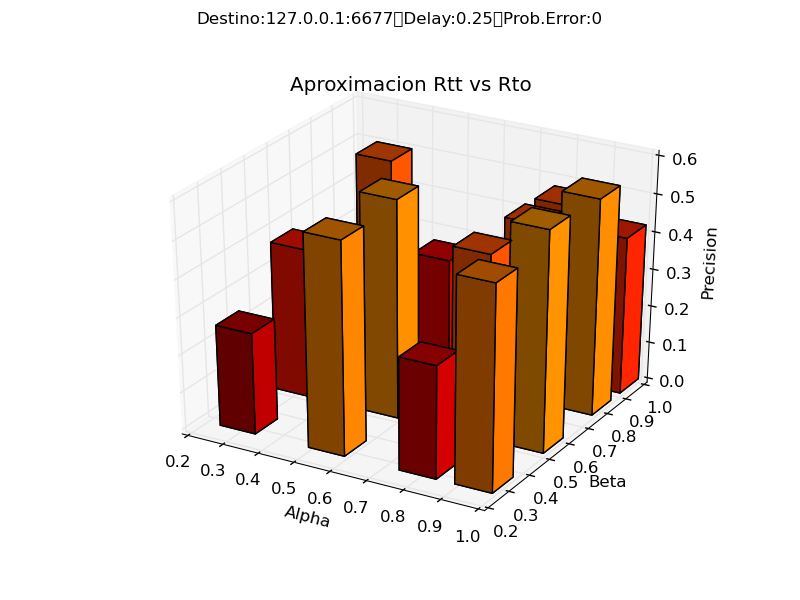
\includegraphics[scale=0.5]{../analisis/graficos_tablas/graficos_en_funcion_de_alfa_y_beta/graficos/rtt_vs_rto.png}
  \caption{Efectividad en la aproximaci\'on del RTO y el RTT Real en funci\'on de $\alpha$ y $\beta$}
	\label{fig:histo-src-sitiotrabajo}
\end{figure}

Observando la figura 1 podemos mencionar que ninguna de las combinaciones de $\alpha$ y $\beta$ super\'o una precisi\'on de 0.6. Sin embargo, observando la altura de las barras, podemos destacar algunas combinaciones que tuvieron resultados por encima de las dem\'as. Estas son:
\begin{itemize}
	\item $\alpha$: 0.5, $\beta$: 0.25
	\item $\alpha$: 0.5, $\beta$: 0.5
	\item $\alpha$: 0.9, $\beta$: 0.5
	\item $\alpha$: 0.9, $\beta$: 0.9
\end{itemize} 

\subsubsection{RTO Estimado}
%	...graficos 3d de las barras con los alfa y beta variados

\begin{figure}[H]
  \centering	
	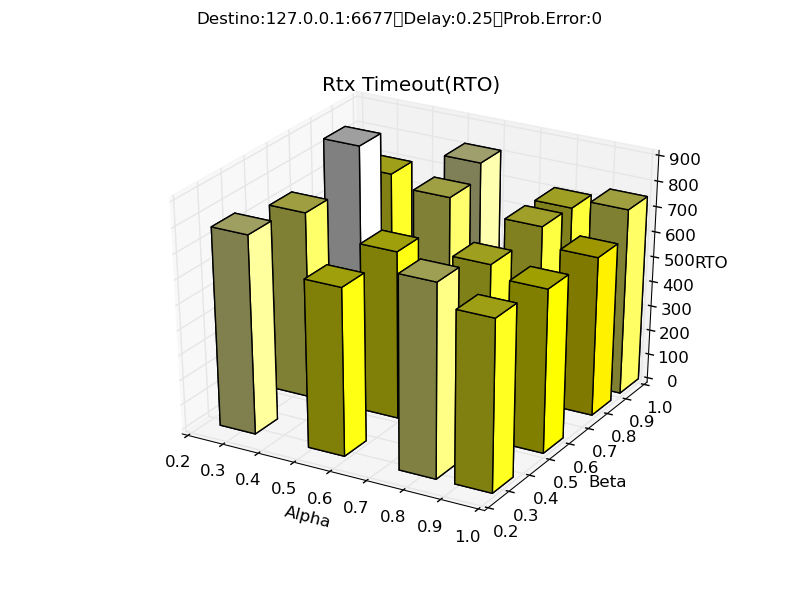
\includegraphics[scale=0.5]{../analisis/graficos_tablas/graficos_en_funcion_de_alfa_y_beta/graficos/rto.png}
  \caption{RTO en funci\'on de $\alpha$ y $\beta$}
	\label{fig:histo-src-sitiotrabajo}
\end{figure}

Este gr\'afico puede complementarse con la figura 1. Mientras m\'as bajos son los valores de RTO para un $\alpha$ y $\beta$ dados, m\'as cercano se encontrar\'a del RTT real. Esto sucede ya que valores de RTO por debajo del RTT real no tendrian sentido. Si reenviamos un paquete antes del tiempo estimado en que recibimos un ACK, el protocolo retransmitir\'ia siempre, relentizando la comunicaci\'on.

Analizando los resultados obtenidos para cada una de las combinaciones destacadas de la secci\'on 3.1.1 podemos mencionar que los RTO estimados se corresponden con los resultados de antes. Las barras, como podemos observar para estas combinaciones, son las que menos altura tienen respecto de las dem\'as, es decir, el RTO es m\'as bajo y por lo tanto m\'as se aproxima al RTT real.

\subsubsection{Cantidad de retransmisiones}
%	...graficos 3d de las barras con los alfa y beta variados
%	no se que decir de esto

\begin{figure}[H]
  \centering	
	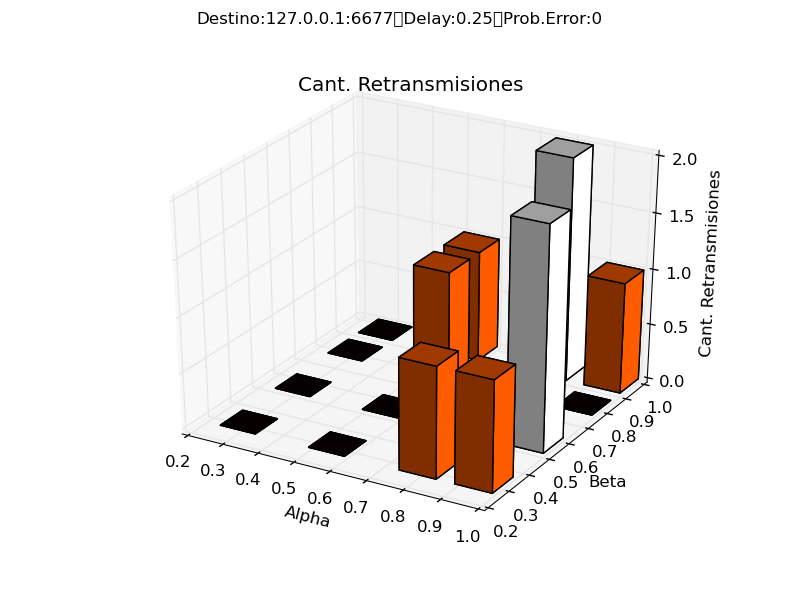
\includegraphics[scale=0.5]{../analisis/graficos_tablas/graficos_en_funcion_de_alfa_y_beta/graficos/retransmisiones.png}
  \caption{Retransmisiones en funci\'on de $\alpha$ y $\beta$}
	\label{fig:histo-src-sitiotrabajo}
\end{figure}







\subsection{Segunda Etapa - Simulacion de problemas de red: Delay y Errores inducidos con probabilidad}
En esta etapa simulamos el comportamiento del protocolo en una red con distintas propiedades. Las propiedades de la red son simuladas con paquetes que se pierden con una probabilidad $p$ y un delay en el reconocimiento de los paquetes (ACK); ambos parámetros pueden simular el congestionamiento de la red, la confiabilidad del canal de comunicación, entre otras cosas. Los experimentos se realizan con las estimaciones de $\alpha$ y $\beta$ encontrados anteriormente.








\subsubsection{Simulación con $\alpha$: 0.5, $\beta$: 0.25}
%%%%%%%%%%%%%%%%%%%%%%%%%%%%%%%%%%%%%%%%%%%%%%%%%%%%%%%%%%%%%%%%%%%%%%%%%%%
%gráficos a comentar


En el gráfico de la figura $4$ podemos observar la cantidad de paquetes retransmitidos para distintos valores de delay y probabilidad de pérdida de paquetes. Se puede observar que, como se esperaba, al aumentar la probabilidad de perder paquetes, fijado un delay, la cantidad de retransmisiones también aumenta. Se puede observar una tendencia al aumento de retransmisiones al aumentar la probabilidad y el delay.

\begin{figure}[H]
  \centering	
	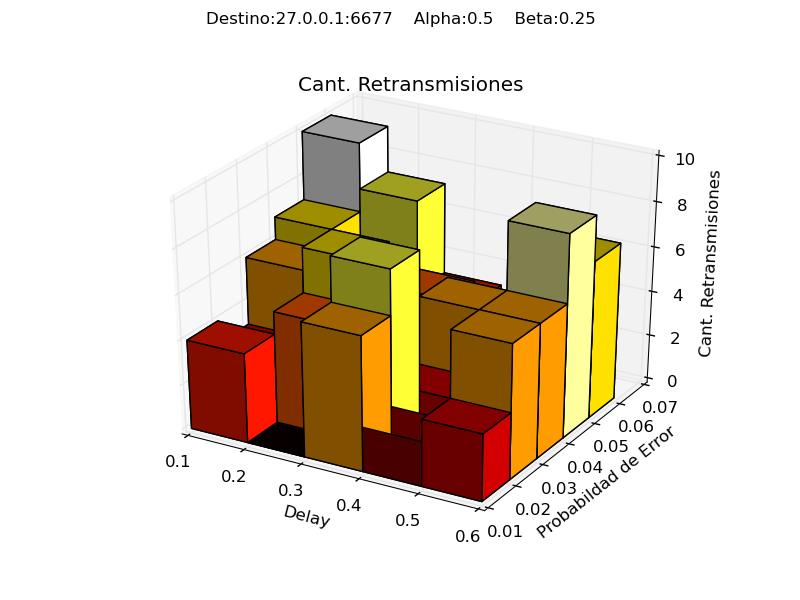
\includegraphics[scale=0.5]{../analisis/graficos_tablas/graficos_en_funcion_de_delay_probaerror/0.5-0.25_2/retransmisiones.png}
  \caption{Retransmisiones en funci\'on del delay y la probabilidad de pérdida de paquetes, para $\alpha$: 0.5, $\beta$: 0.25}
	\label{fig:histo-src-sitiotrabajo}
\end{figure}

En la figura $5$ están los datos del experimento que se realizó para analizar el impacto en el cálculo del RTO al variar el delay y la probabilidad de pérdidas de paquetes. Podemos notar en el gráfico que el valor del RTO aumenta cuando también lo hace el delay y pa probabilidad. El mayor valor del RTO se encuentra en delay $= 0.3$ y probabilidad $= 0.02$ , pero mirando la distribución de los demás valores, éste parece ser un valor atípico.

\begin{figure}[H]
  \centering	
	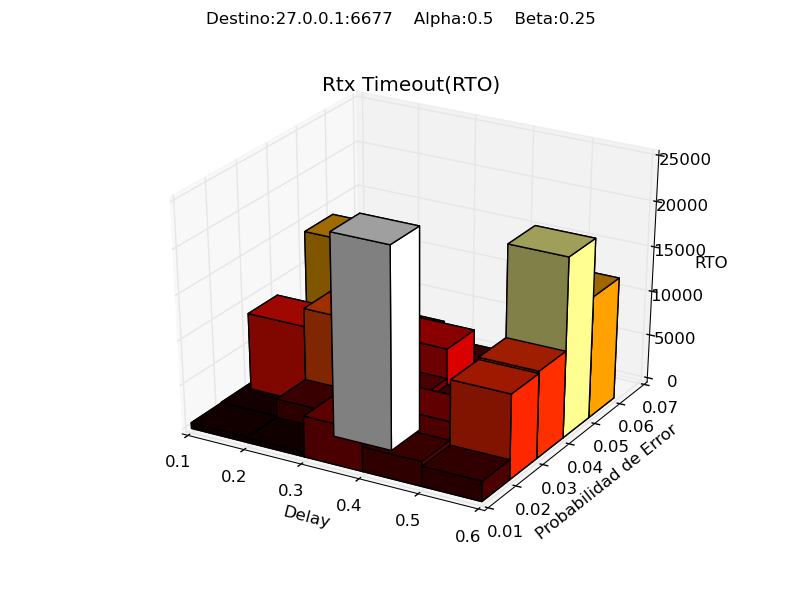
\includegraphics[scale=0.5]{../analisis/graficos_tablas/graficos_en_funcion_de_delay_probaerror/0.5-0.25_2/rto.png}
  \caption{RTO en función del delay y la probabilidad de pérdida de paquetes, para $\alpha$: 0.5, $\beta$: 0.25}
	\label{fig:histo-src-sitiotrabajo}
\end{figure}

En la figura $6$ podemos observar la relación entre el RTO y el RTT en función del delay y la probabilidad de error. Claramente al aumentar el delay y la probabilidad, la precisión desciende. Puede verse también que si se fija el delay, al disminuir la probabilidad de error, disminuye la precición. Este análisis es importante debido a que el RTO define cuando un paquete se puede dar por perdido. Si el RTO es demasiado grande, se tarda en dar por perdido un paquete, mientras que si es muy chico, el paquete se da por perdido demasiado rápido. Concluimos que tener una red más confiable (sin congestión, por ejemplo) ayuda al cálculo del RTO.

\begin{figure}[H]
  \centering	
	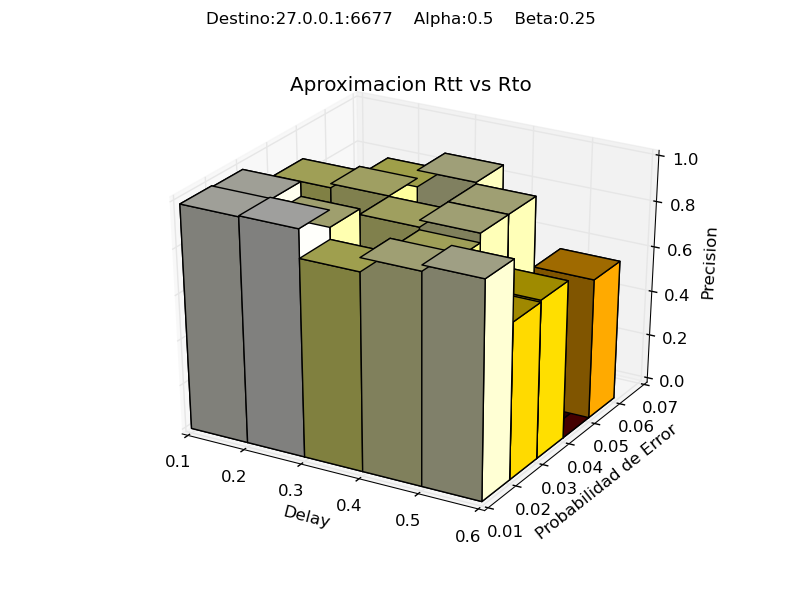
\includegraphics[scale=0.5]{../analisis/graficos_tablas/graficos_en_funcion_de_delay_probaerror/0.5-0.25_2/rtt_vs_rto.png}
  \caption{Diferencia entre RTT y RTO en funci\'on del delay y la probabilidad de pérdida de paquetes, para $\alpha$: 0.5, $\beta$: 0.25}
	\label{fig:histo-src-sitiotrabajo}
\end{figure}











\subsubsection{Simulación con $\alpha$: 0.5, $\beta$: 0.5}
%%%%%%%%%%%%%%%%%%%%%%%%%%%%%%%%%%%%%%%%%%%%%%%%%%%%%%%%%%%%%%%%%%%%%%%%%%%
%gráficos a comentar

Llevamos a cabo un experimento para medir la cantidad de retransmisiones en función del delay y la probabilidad de pérdida de los paquetes. Los resultados se encuentran en el gráfico de la figura $7$. Podemos ver que la distribución de la cantidad de retransmisiones es bastante estática, es decir, no hay cambios bruscos en la cantidad de retransmisiones al mover los parámetros. Aún así, puede observarse que cuando el delay se encuentra entre $0.1$ y $0.3$ y la probabilidad entre $0.01$ y $0.03$ se alcanza una distribución con una media menor. Podemos concluir entonces que la cantidad de retransmisiones que ocurren disminuyen al disminuir los parámetros mencionados.

\begin{figure}[H]
  \centering	
	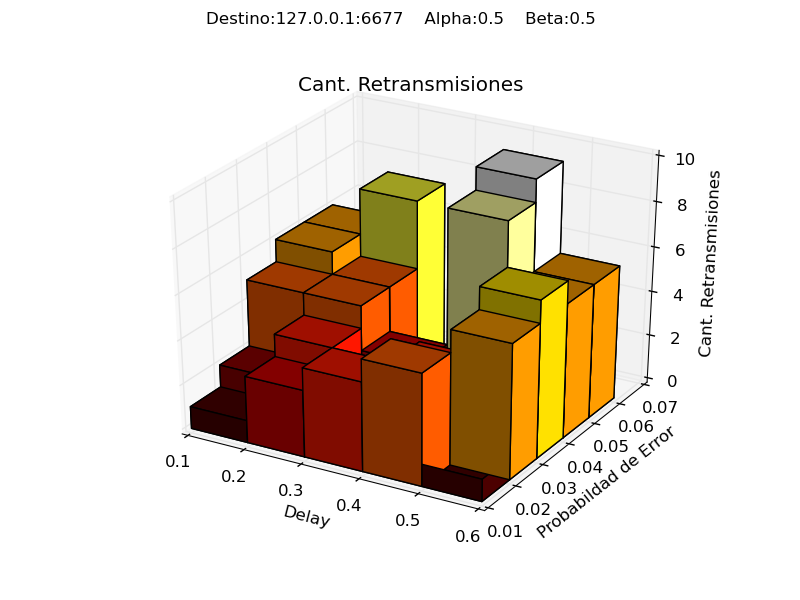
\includegraphics[scale=0.5]{../analisis/graficos_tablas/graficos_en_funcion_de_delay_probaerror/0.5-0.5/retransmisiones.png}
  \caption{Retransmisiones en funci\'on del delay y la probabilidad de pérdida de paquetes, para $\alpha$: 0.5, $\beta$: 0.5}
	\label{fig:histo-src-sitiotrabajo}
\end{figure}

En el gráfico de la figura $8$ se volcaron los datos obtenidos al medir RTO estimado por el protocolo en función del delay y la probailidad de error. Podemos ver que para la mayoría de los valores el RTO es menor a los $10000$. Los valores de RTO mayores se encuentran con un delay de $0.5$ y una probabilidad de $0.03$. Se puede observar que el RTO medio para un delay de $0.5$ es mayor a los otros. La distribución de valores del RTO no es demasiado clara, aunque parece ser que tener un mayor delay aumenta el RTO. Esta última observación es esperable, ya que al aumentar el delay, el RTT parec ser mayor, y entonces, el RTO debe también aumentar.

\begin{figure}[H]
  \centering	
	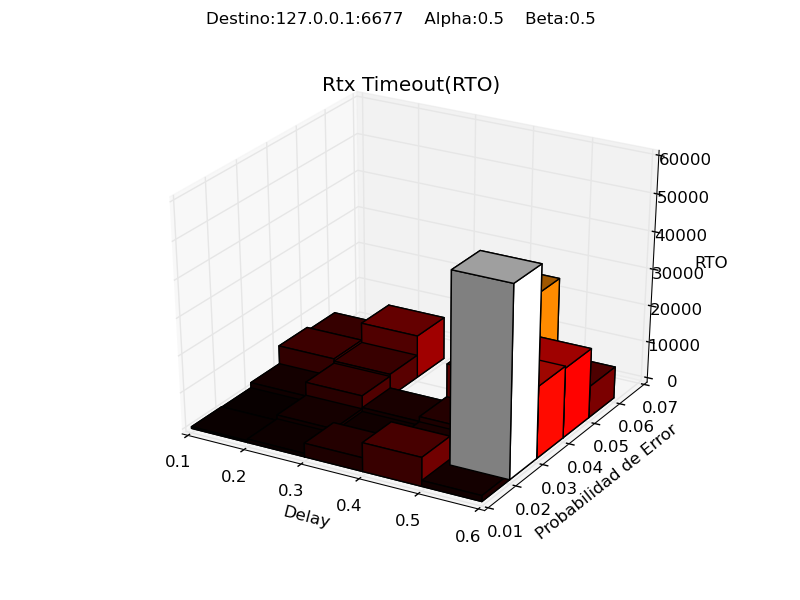
\includegraphics[scale=0.5]{../analisis/graficos_tablas/graficos_en_funcion_de_delay_probaerror/0.5-0.5/rto.png}
  \caption{RTO en función del delay y la probabilidad de pérdida de paquetes, para $\alpha$: 0.5, $\beta$: 0.5}
	\label{fig:histo-src-sitiotrabajo}
\end{figure}

En la figura $9$ podemos ver la relación entre RTT y RTO al variar la probabilidad de error y el delay al reconocer los paquetes (envio del ACK). Como con los demás valores de $\alpha$ y $\beta$ con los que se llevo a cabo este experimento, un aumento de delay y probabilidad se traduce en una disminución de la precisión. 

\begin{figure}[H]
  \centering	
	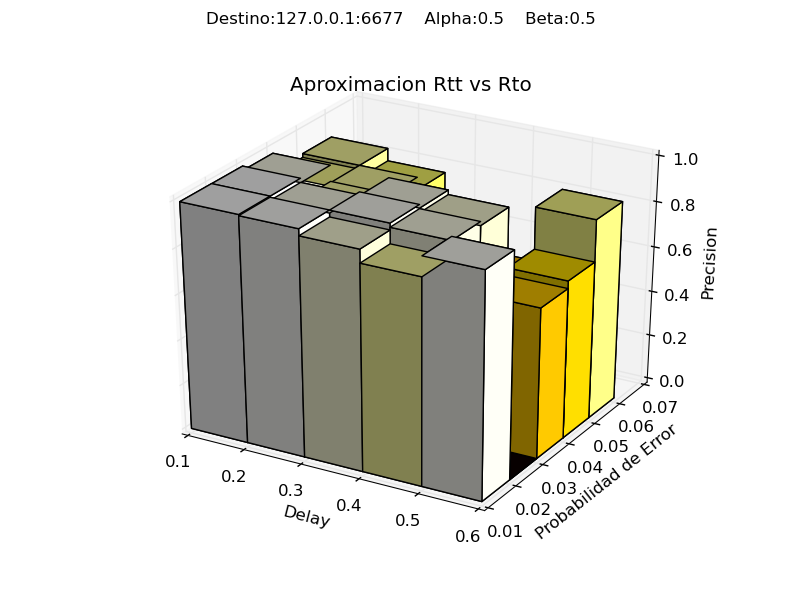
\includegraphics[scale=0.5]{../analisis/graficos_tablas/graficos_en_funcion_de_delay_probaerror/0.5-0.5/rtt_vs_rto.png}
  \caption{Diferencia entre RTT y RTO en funci\'on del delay y la probabilidad de pérdida de paquetes, para $\alpha$: 0.5, $\beta$: 0.5}
	\label{fig:histo-src-sitiotrabajo}
\end{figure}









\subsubsection{Simulación con $\alpha$: 0.9, $\beta$: 0.5}
%%%%%%%%%%%%%%%%%%%%%%%%%%%%%%%%%%%%%%%%%%%%%%%%%%%%%%%%%%%%%%%%%%%%%%%%%%%
%gráficos a comentar

En el gráfico de la figura $10$ están representados los datos obtenidos al medir la cantidad de retransmisiones en función de las probabilidad de perder paquetes y el delay al enviar los ACK. Podemos ver que al aumentar el delay y la probabilidad, la cantidad de paquetes retransmitidos aumenta. Como se explicó anteriormente esto tiene sentido, ya que el aumento de ambos parámetros indica que más paquetes se pierden y se tarda más en reconocer los paquetes que arrivan, lo que puede ocasionar un time out. Podemos ver también que, fijando un delay, un aumento de la probabilidad de pérdida de paquetes genera un aumento en la cantidad de retransmisiones.

\begin{figure}[H]
  \centering	
	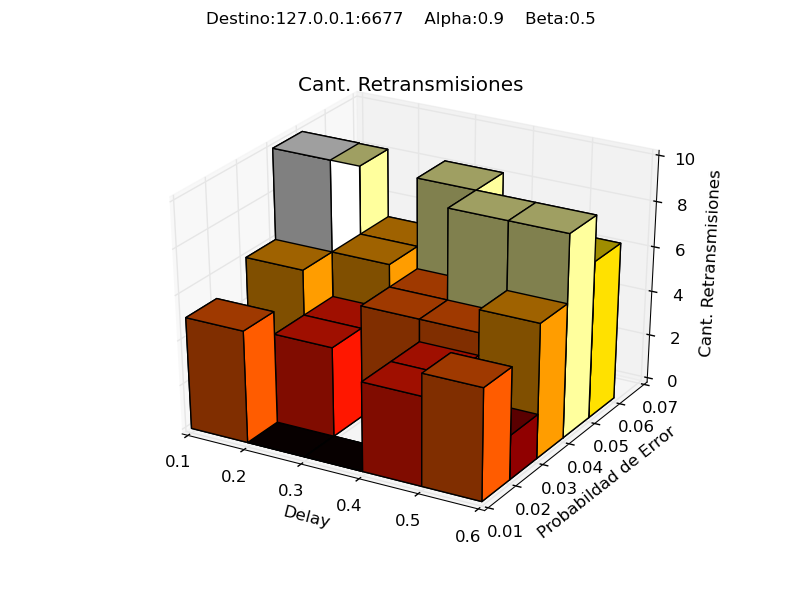
\includegraphics[scale=0.5]{../analisis/graficos_tablas/graficos_en_funcion_de_delay_probaerror/0.9-0.5/retransmisiones.png}
  \caption{Retransmisiones en funci\'on del delay y la probabilidad de pérdida de paquetes, para $\alpha$: 0.9, $\beta$: 0.5}
	\label{fig:histo-src-sitiotrabajo}
\end{figure}

En el gráfico de la figura $11$ podemos ver el impacto de la variación de la probabilidad de pérdida de paquetes y el delay en el cálculo del RTO. Podemos ver que, para la gran mayoría de los valores de los parámetros, el RTO no alcanza los $50000$ y hay un máximo en delay $0.5$ y probabilidad $0.06$. 


\begin{figure}[H]
  \centering	
	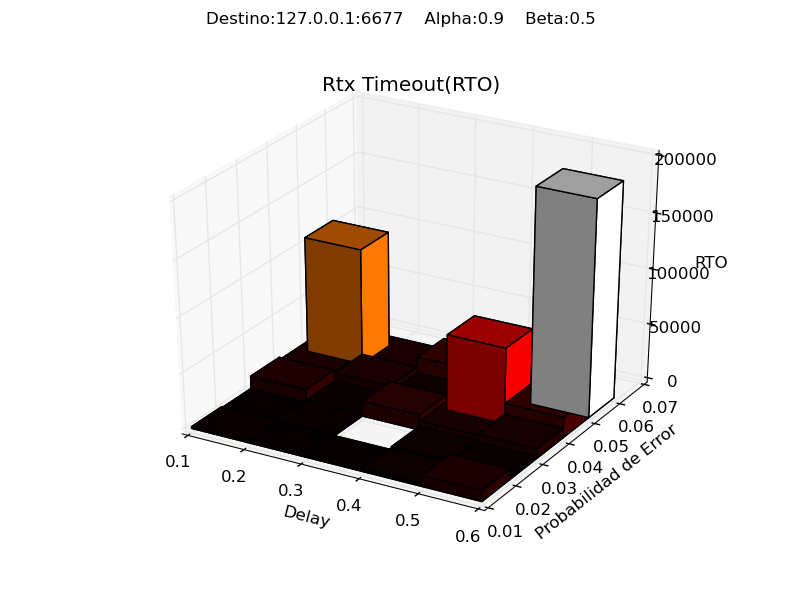
\includegraphics[scale=0.5]{../analisis/graficos_tablas/graficos_en_funcion_de_delay_probaerror/0.9-0.5/rto.png}
  \caption{RTO en función del delay y la probabilidad de pérdida de paquetes, para $\alpha$: 0.9, $\beta$: 0.5}
	\label{fig:histo-src-sitiotrabajo}
\end{figure}

En el gráfico de la figura $12$ podemos ver la relación entre el RTO medido en el protocolo y el RTT entre el cliente y el servidor, en función del delay y la probabilidad de pérdida de los paquetes. Como en los experimentos en que medimos la misma relación con distintos $\alpha$ y $\beta$, al aumentar el delay y la probabilidad, se observa una precisión menor. Pero también, comparando con los experimento anteriores, notamos que la variación es menor pronunciada.

\begin{figure}[H]
  \centering	
	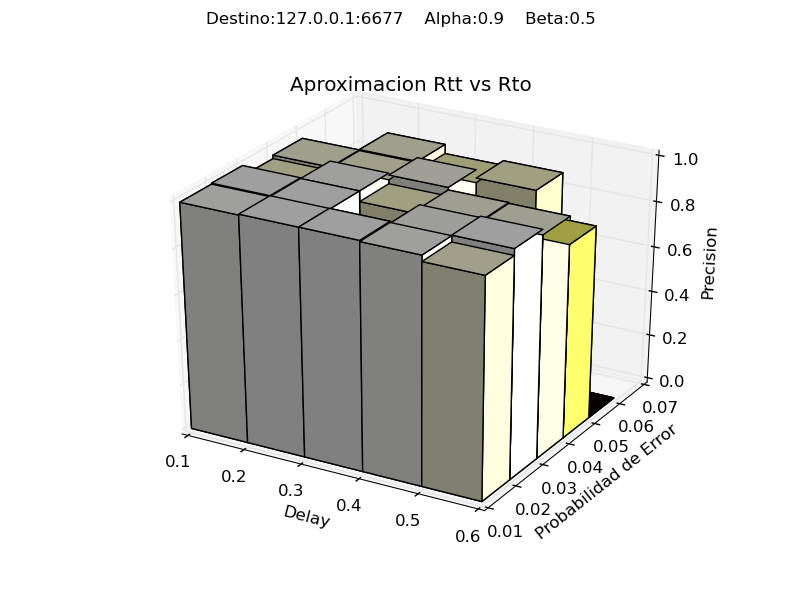
\includegraphics[scale=0.5]{../analisis/graficos_tablas/graficos_en_funcion_de_delay_probaerror/0.9-0.5/rtt_vs_rto.png}
  \caption{Diferencia entre RTT y RTO en funci\'on del delay y la probabilidad de pérdida de paquetes, para $\alpha$: 0.9, $\beta$: 0.5}
	\label{fig:histo-src-sitiotrabajo}
\end{figure}











\subsubsection{Simuación con $\alpha$: 0.9, $\beta$: 0.9}
%%%%%%%%%%%%%%%%%%%%%%%%%%%%%%%%%%%%%%%%%%%%%%%%%%%%%%%%%%%%%%%%%%%%%%%%%%%
%gráficos a comentar

En la figura $13$ podemos ver la relación entre la cantidad de retransmisiones y la probabilidad de error y el delay. Para estos valores de $\alpha$ y $\beta$ observamos que la relación entre las variables no es tan clara como en experimentos similares anteriores. Si eliminamos algunos datos atípicos (por ejemplo delay $0.4$ y probabilidad $0.02$), se puede ver que la relación es más clara, es decir, el aumento de delay y probabilidad parece estar correlacionado con un aumento en la cantidad de paquetes que deben ser retransmitidos.

\begin{figure}[H]
  \centering	
	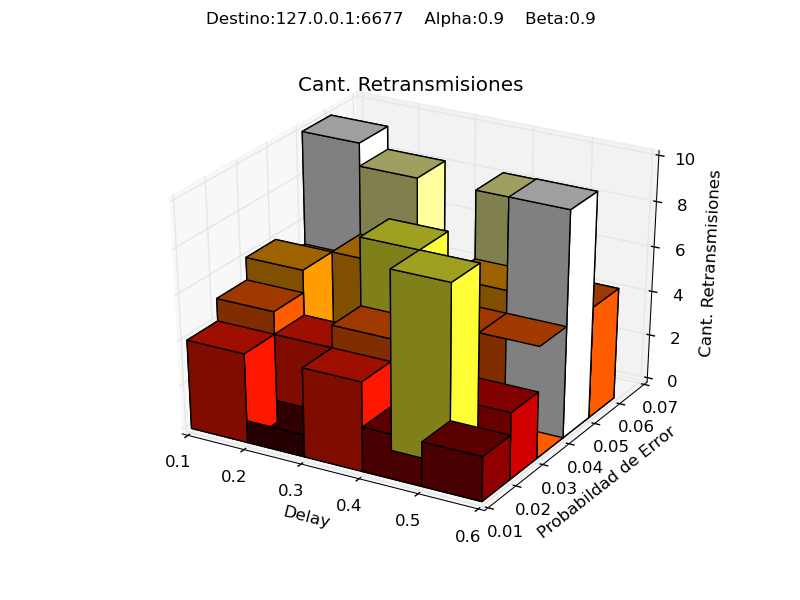
\includegraphics[scale=0.5]{../analisis/graficos_tablas/graficos_en_funcion_de_delay_probaerror/0.9-0.9/retransmisiones.png}
  \caption{Retransmisiones en funci\'on del delay y la probabilidad de pérdida de paquetes, para $\alpha$: 0.9, $\beta$: 0.9}
	\label{fig:histo-src-sitiotrabajo}
\end{figure}

En el gráfico de la figura $14$ se muestra la relación medida experimentalmente entre el RTO y el delay y la probabilidad de errores. Podemos ver que se alcanza un máximo en delay $0.3$ y probabilidad de error $0.03$. Notamos que este dato es un valor atípico, ya que su magnitud es mucho mayor a los demás datos. No podemos observar una relación claraen este experimento.

\begin{figure}[H]
  \centering	
	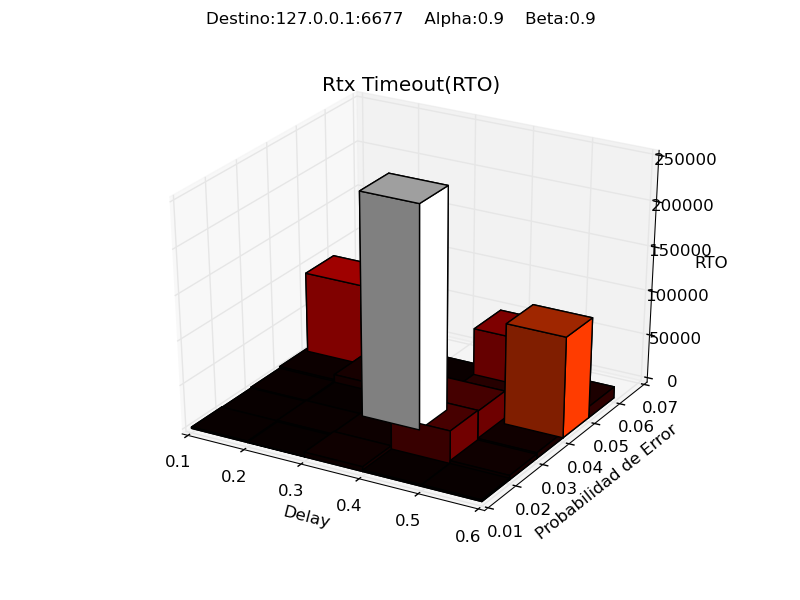
\includegraphics[scale=0.5]{../analisis/graficos_tablas/graficos_en_funcion_de_delay_probaerror/0.9-0.9/rto.png}
  \caption{RTO en función del delay y la probabilidad de pérdida de paquetes, para $\alpha$: 0.9, $\beta$: 0.9}
	\label{fig:histo-src-sitiotrabajo}
\end{figure}

En el gráfico de la figura $15$ están los datos obtenidos experimentalmente sobre la precisión del RTO en relación al RTT, al variar el delay y la probabilidad de error. Podemos ver que al aumentar estos dos valores la precisión parece disminuir. También notamos que la relación no es muy evidente, como lo es para otros $\alpha$ y $\beta$.

\begin{figure}[H]
  \centering	
	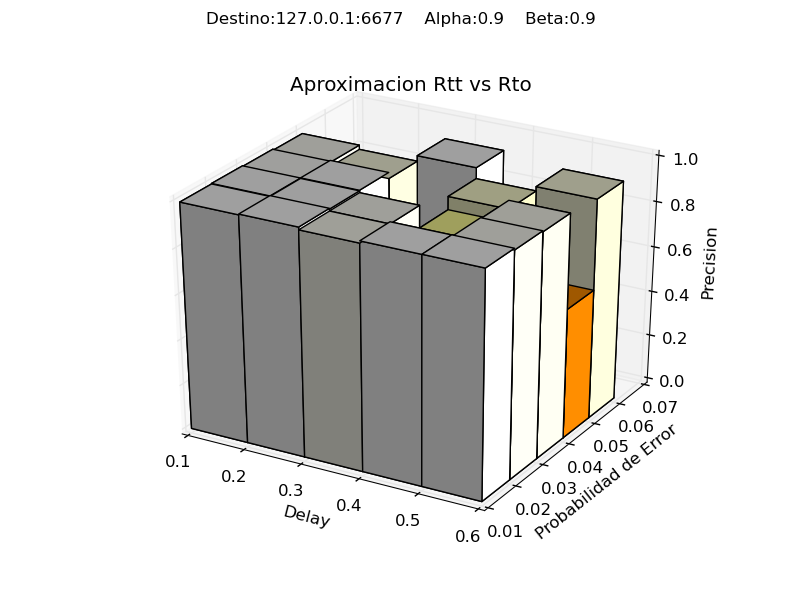
\includegraphics[scale=0.5]{../analisis/graficos_tablas/graficos_en_funcion_de_delay_probaerror/0.9-0.9/rtt_vs_rto.png}
  \caption{Diferencia entre RTT y RTO en funci\'on del delay y la probabilidad de pérdida de paquetes, para $\alpha$: 0.9, $\beta$: 0.9}
	\label{fig:histo-src-sitiotrabajo}
\end{figure}

